% !TEX encoding = UTF-8 Unicode
\documentclass[a4paper,12pt]{report}

\usepackage[utf8]{inputenc}
\usepackage[T1]{fontenc}
\usepackage[french]{babel}
\usepackage{graphicx}
\usepackage{geometry}
\usepackage{float}
\usepackage{amsmath}
\usepackage{enumitem}
\usepackage{booktabs}
\usepackage{url}
\usepackage{caption}
\usepackage{subcaption}
\usepackage{xcolor}
\usepackage{titlesec}
\usepackage{fancyhdr}
\usepackage[colorlinks=true,linkcolor=blue!60!black,urlcolor=blue!60!black,citecolor=blue!60!black]{hyperref}

\geometry{margin=2.5cm}
\graphicspath{{figures/}{figures/captures/}}

\definecolor{accent}{RGB}{31,78,121}
\definecolor{accentlight}{RGB}{46,117,182}

\pagestyle{fancy}
\fancyhf{}
\fancyhead[L]{\small\textcolor{accent}{Plateforme événements--prestataires}}
\fancyhead[R]{\small\textcolor{gray}{\thepage}}
\renewcommand{\headrulewidth}{0.4pt}

\titleformat{\chapter}[display]
  {\normalfont\LARGE\bfseries\color{accent}}
  {\chaptertitlename\ \thechapter}{10pt}{\Huge}
\titleformat{\section}
  {\normalfont\large\bfseries\color{accentlight}}
  {\thesection}{1em}{}
\titleformat{\subsection}
  {\normalfont\normalsize\bfseries\color{black}}
  {\thesubsection}{1em}{}

\title{%
  \textbf{\textcolor{accent}{Plateforme intelligente de mise en relation\\
  Événements -- Prestataires}}\\[0.5cm]
  \large Rapport de projet de fin d'études\\[0.3cm]
  \normalsize Année universitaire 2025--2026%
}

\author{%
  Yasmine Yedes \and
  Siwar Sahraoui \and
  Malek Sfeihi%
}

\date{}

\begin{document}

\maketitle
\thispagestyle{empty}

\chapter*{Remerciements}
\addcontentsline{toc}{chapter}{Remerciements}

\noindent
Nous tenons à exprimer notre gratitude à notre encadrant pour son accompagnement, ses conseils méthodologiques et la disponibilité dont il a fait preuve tout au long de ce projet de fin d'études.

\vspace{1em}

\noindent
Nous remercions également les membres du jury pour le temps qu'ils consacreront à l'examen de ce travail et pour leurs questions qui contribueront à en enrichir la lecture.

\chapter*{Résumé}
\addcontentsline{toc}{chapter}{Résumé}

\noindent
Ce rapport présente la conception et la réalisation d'une plateforme web destinée à faciliter la mise en relation entre organisateurs d'événements et prestataires (salles, traiteurs, animation, etc.). Les montants monétaires sont exprimés en \textbf{dinars tunisiens} (DT) dans l'interface. Le système couvre l'ensemble du cycle métier : gestion des comptes et des rôles, création d'événements, catalogue des prestataires validés, demandes et traitement des réservations, administration, ainsi qu'un module d'aide à la décision fondé sur des scores de compatibilité, une estimation de probabilité d'acceptation et une explicabilité des recommandations.

\vspace{0.5em}

\noindent
La solution repose sur une architecture moderne : API REST sous Spring Boot, interface utilisateur Angular, persistance PostgreSQL, authentification et autorisation par rôles (JWT). Le module d'intelligence artificielle combine un microservice \textbf{FastAPI} (Python), où sont implémentés le scoring et l'explicabilité, et une orchestration côté Spring Boot qui agrège les données et sécurise les accès ; l'interface organisateur consomme les résultats via l'API REST exposée par le backend.

\vspace{1em}

\noindent
\textbf{Mots-clés :} événementiel, mise en relation, Spring Boot, Angular, PostgreSQL, Python, FastAPI, intelligence artificielle, UML.

\chapter*{Abstract}
\addcontentsline{toc}{chapter}{Abstract}

\noindent
This report presents the design and implementation of a web platform connecting event organizers with service providers. The system covers the full business scope: account and role management, event lifecycle, validated provider catalog, reservation workflows, administration, and a decision-support module based on compatibility scoring, acceptance probability estimates, and explainable recommendations.

\vspace{0.5em}

\noindent
The solution uses a REST API (Spring Boot), an Angular SPA, PostgreSQL persistence, and JWT-based role security. The decision-support layer combines a Python FastAPI microservice (scoring and explainability) with orchestration and authorization in Spring Boot; the organizer UI consumes the unified REST surface.

\vspace{1em}

\noindent
\textbf{Keywords:} event management, matching, Spring Boot, Angular, PostgreSQL, artificial intelligence, software design, UML.

\tableofcontents
\listoffigures
\newpage

%==================================================
\chapter*{Introduction générale}
\addcontentsline{toc}{chapter}{Introduction générale}

\noindent
L'économie des événements repose sur une coordination rapide entre besoins exprimés (type de manifestation, date, budget, capacité) et offres disponibles (profils prestataires validés). Les échanges informels et l'absence d'outil commun peuvent entraîner des refus répétés, une faible adéquation entre demande et proposition et une traçabilité limitée des interactions.

\vspace{0.5em}

\noindent
Le présent document décrit la démarche menée pour concevoir et réaliser une plateforme répondant à cette problématique. Il traite le projet dans son ensemble : besoins, modélisation, architecture, module d'intelligence artificielle, implémentation et sécurité.

\vspace{0.5em}

\noindent
Après une présentation du contexte (chapitre~\ref{chap:presentation}), l'analyse des besoins est développée au chapitre~\ref{chap:besoins}. Le chapitre~\ref{chap:ia} détaille le module d'intelligence artificielle. Les modèles UML sont présentés au chapitre~\ref{chap:uml}. L'architecture technique et la réalisation logicielle sont abordées aux chapitres~\ref{chap:archi} et~\ref{chap:real}. Des captures d'interface illustrent le produit au chapitre~\ref{chap:captures}. Les aspects de sécurité et le bilan ferment le rapport.

%==================================================
\chapter{Présentation générale du projet}
\label{chap:presentation}

\section{Contexte et problématique}

L'organisation d'événements est un secteur dynamique. Dans la vie réelle, une personne qui souhaite fêter un anniversaire ou un mariage s'adresse souvent à un \textbf{organisateur professionnel} : celui-ci formalise le besoin (type de fête, nombre d'invités, budget en dinars, thème ou préférences) et coordonne ensuite plusieurs prestataires (traiteur, DJ, décoration, etc.). Notre plateforme numérise ce rôle d'organisateur en lui offrant un catalogue contrôlé, des demandes structurées et une aide au choix des prestataires ; le client final peut être représenté dans le système par le \textbf{projet d'événement} que l'organisateur crée.

La mise en relation entre porteurs de projet et prestataires demeure souvent fragmentée lorsqu'il n'existe pas d'outil commun : messageries disparates, critères mal alignés sur les capacités et le budget, peu de vision consolidée des demandes en cours.

Les difficultés que vise à réduire la plateforme incluent notamment :
\begin{itemize}[leftmargin=*]
  \item une adéquation insuffisante entre le type d'événement et les prestataires sollicités ;
  \item des refus liés à une capacité ou un budget inadaptés ;
  \item le besoin d'une aide à la décision (classement, scores, estimation des chances d'acceptation), assuré par le module d'intelligence artificielle ;
  \item la nécessité de suivre les demandes de réservation de façon structurée.
\end{itemize}

\section{Objectifs et périmètre}

La plateforme offre un parcours complet pour les organisateurs, les prestataires et les administrateurs. Elle combine gestion métier classique (événements, catalogue, réservations, validation des profils) et fonctionnalités intelligentes : recommandation et classement des prestataires, scores de compatibilité, estimation de probabilité d'acceptation et messages d'explicabilité associés aux résultats.

\section{Technologies retenues}

\begin{itemize}[leftmargin=*]
  \item \textbf{Backend :} Java~17, Spring Boot~3 (API REST, Spring Security, JWT, client HTTP \texttt{RestClient} vers le microservice IA).
  \item \textbf{Frontend :} Angular (SPA, intercepteur JWT, garde par rôle).
  \item \textbf{Données :} PostgreSQL, JPA/Hibernate (utilisateur, événement, profil prestataire, réservation).
  \item \textbf{Module IA :} Python~3, FastAPI (\texttt{ai/python-service}) — scoring et explicabilité ; évolution possible vers scikit-learn sans changer le contrat exposé au backend.
  \item \textbf{Sécurité :} BCrypt, contrôle d'accès par rôle.
\end{itemize}

%==================================================
\chapter{Analyse des besoins}
\label{chap:besoins}

\section{Besoins fonctionnels côté organisateur}

\begin{itemize}[leftmargin=*]
  \item authentification ; création, lecture, mise à jour et suppression des événements (type, date, nombre de participants, budget, préférences) ;
  \item consultation du catalogue des prestataires validés ; envoi et suivi des demandes de réservation ;
  \item obtention d'un classement ou de recommandations de prestataires ; consultation d'un score de compatibilité et d'une estimation de probabilité d'acceptation ; lecture d'un court texte récapitulant les critères ayant le plus influencé le classement (explicabilité).
\end{itemize}

\section{Besoins fonctionnels côté prestataire}

\begin{itemize}[leftmargin=*]
  \item profil métier (capacités, types d'événements couverts, tarification, éventuellement notes ou indicateurs) soumis à validation administrative ;
  \item traitement des demandes reçues (acceptation ou refus).
\end{itemize}

\section{Besoins fonctionnels côté administration}

\begin{itemize}[leftmargin=*]
  \item tableau de bord, validation des profils prestataires, gestion des comptes utilisateurs ;
  \item supervision des indicateurs globaux (utilisateurs, réservations, files d'attente de validation).
\end{itemize}

\section{Synthèse}

Les besoins ci-dessus se traduisent par une application unifiée : parcours utilisateurs, persistance des entités métier, exposition des services de recommandation et affichage des résultats dans l'interface organisateur.

\section{Besoins non fonctionnels}

\begin{itemize}[leftmargin=*]
  \item \textbf{Performance :} temps de réponse convenable pour les opérations courantes ; le calcul enrichi par le module intelligent vise un ordre de grandeur inférieur à trois secondes sous charge nominale.
  \item \textbf{Sécurité :} stockage sûr des secrets d'authentification, contrôle d'accès par rôle, déploiement en HTTPS en production.
  \item \textbf{Fiabilité et transparence :} traçabilité des critères pris en compte dans les scores et les classements.
\end{itemize}

%==================================================
\chapter{Conception du module d'intelligence artificielle}
\label{chap:ia}

\section{Rôle du module}

Le module d'intelligence artificielle apporte une aide à la décision à l'organisateur avant l'envoi formel d'une demande de réservation : il classe les prestataires éligibles (profils validés et comptes actifs), attribue un score de compatibilité entre l'événement choisi et chaque offre, et estime une probabilité d'acceptation en combinant ce score avec un indicateur issu de l'historique des réservations (taux d'acceptation sur les demandes déjà tranchées).

\section{Données d'entrée et de sortie}

Les entrées regroupent les attributs de l'événement (type, date, nombre de participants, budget, préférences structurées ou vectorisées si nécessaire), les attributs du profil prestataire (capacité, types acceptés, prix minimum) et, le cas échéant, un historique des réservations (taux d'acceptation par catégorie).

Les sorties fournissent une liste ordonnée d'identifiants de prestataires ; pour chaque candidat retenu : une valeur de score, une probabilité estimée lorsque le modèle le permet, et un court texte d'explication mettant en avant les critères dominants.

\section{Interface logicielle}

Le diagramme de classes (figure~\ref{fig:cl}) introduit une interface \texttt{IARecommendationService} et un objet résultat \texttt{RecommendationScore}. Dans l'implémentation, le contrat est matérialisé par le service Spring \texttt{RecommendationServiceImpl}, le client HTTP \texttt{PythonRecommendationClient} et un enregistrement de transfert \texttt{RecommendationScoreResponse} (identifiant prestataire, nom commercial, score entier sur 100, probabilité bornée entre 0 et 1, texte d'explication).

\section{Modèle de calcul implémenté}

Pour chaque prestataire du catalogue administré, quatre sous-scores normalisés entre 0 et 100 sont calculés puis combinés linéairement :
\begin{itemize}[leftmargin=*]
  \item \textbf{Type d'événement :} correspondance insensible à la casse entre le type saisi pour l'événement et l'ensemble des types acceptés par le prestataire.
  \item \textbf{Capacité :} adéquation entre le nombre de participants et la fourchette \texttt{minCapacity}--\texttt{maxCapacity} ; pénalisation progressive si la taille du groupe sort de l'intervalle.
  \item \textbf{Budget :} comparaison du budget de l'événement au prix minimum du prestataire (prise en compte d'une marge confortable lorsque le budget dépasse nettement le minimum).
  \item \textbf{Historique :} proportion de réservations acceptées parmi les réservations déjà acceptées ou refusées pour ce prestataire ; en l'absence d'historique tranché, une valeur neutre évite de pénaliser les nouveaux profils.
\end{itemize}

Les pondérations appliquées sont $0{,}30$ (type), $0{,}25$ (capacité), $0{,}25$ (budget) et $0{,}20$ (historique). Le score de compatibilité affiché est la moyenne pondérée arrondie sur $[0,100]$. La probabilité d'acceptation affichée est une fusion convexifiée du score normalisé et du taux historique (coefficients $0{,}62$ et $0{,}38$), puis bornée pour éviter des valeurs extrêmes non interprétables.

Le calcul effectif est implémenté dans le projet Python (\texttt{ai/python-service}, module \texttt{scoring.py}), exposé par une API \textbf{FastAPI}. Cette séparation permet d'évoluer vers des modèles d'apprentissage (scikit-learn, réseaux de neurones, etc.) sans modifier le frontend ni le contrat REST public du backend Java.

\section{Exposition API et interface utilisateur}

L'endpoint \texttt{GET /api/recommendations/events/\{eventId\}} est réservé au rôle organisateur ; Spring Boot vérifie que l'événement appartient à l'utilisateur, agrège les données métier puis appelle le service FastAPI en \texttt{POST /api/v1/recommendations/score}. La réponse renvoyée au navigateur est une liste triée par score décroissant. Côté Angular, la route \texttt{/organizer/recommendations} propose le choix de l'événement et affiche le tableau de classement avec score, probabilité et texte explicatif.

Une désactivation du service Python est possible via configuration (\texttt{recommendation.python.enabled=false}) : le même modèle de calcul est alors exécuté en Java (\texttt{LocalRecommendationScorer}) pour les environnements sans runtime Python.

\section{Explicabilité}

Les phrases affichées sont générées à partir des valeurs des sous-scores : elles mettent en avant les critères forts (type couvert, capacité adaptée, budget confortable, historique favorable) ou les écarts sensibles (type absent du profil, capacité ou budget mal alignés, historique de refus), ce qui répond au besoin de transparence vis-à-vis de l'organisateur.

%==================================================
\chapter{Modélisation UML}
\label{chap:uml}

Les figures suivantes modélisent l'ensemble fonctionnel de la plateforme : parcours métier, réservations, administration et interactions avec le module d'intelligence artificielle décrit au chapitre~\ref{chap:ia}.

\section{Diagramme de cas d'utilisation}

\begin{figure}[H]
  \centering
  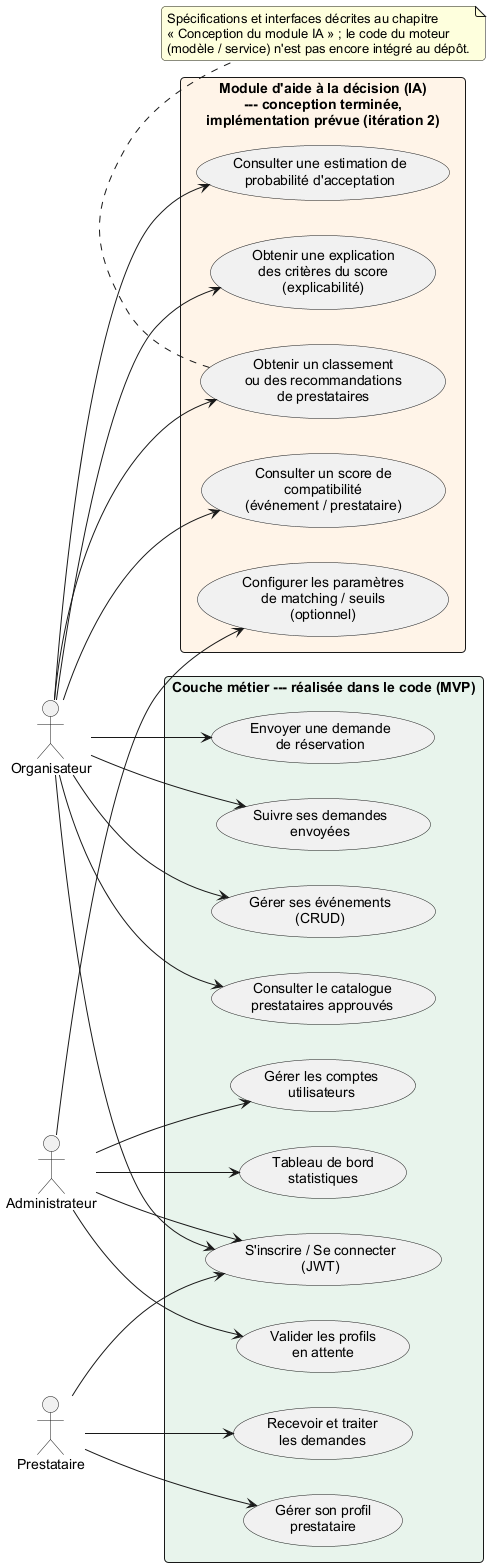
\includegraphics[width=\textwidth]{cas_utilisation.png}
  \caption{Cas d'utilisation de la plateforme (métier et module d'intelligence artificielle)}
  \label{fig:uc}
\end{figure}

\section{Diagramme de classes}

\begin{figure}[H]
  \centering
  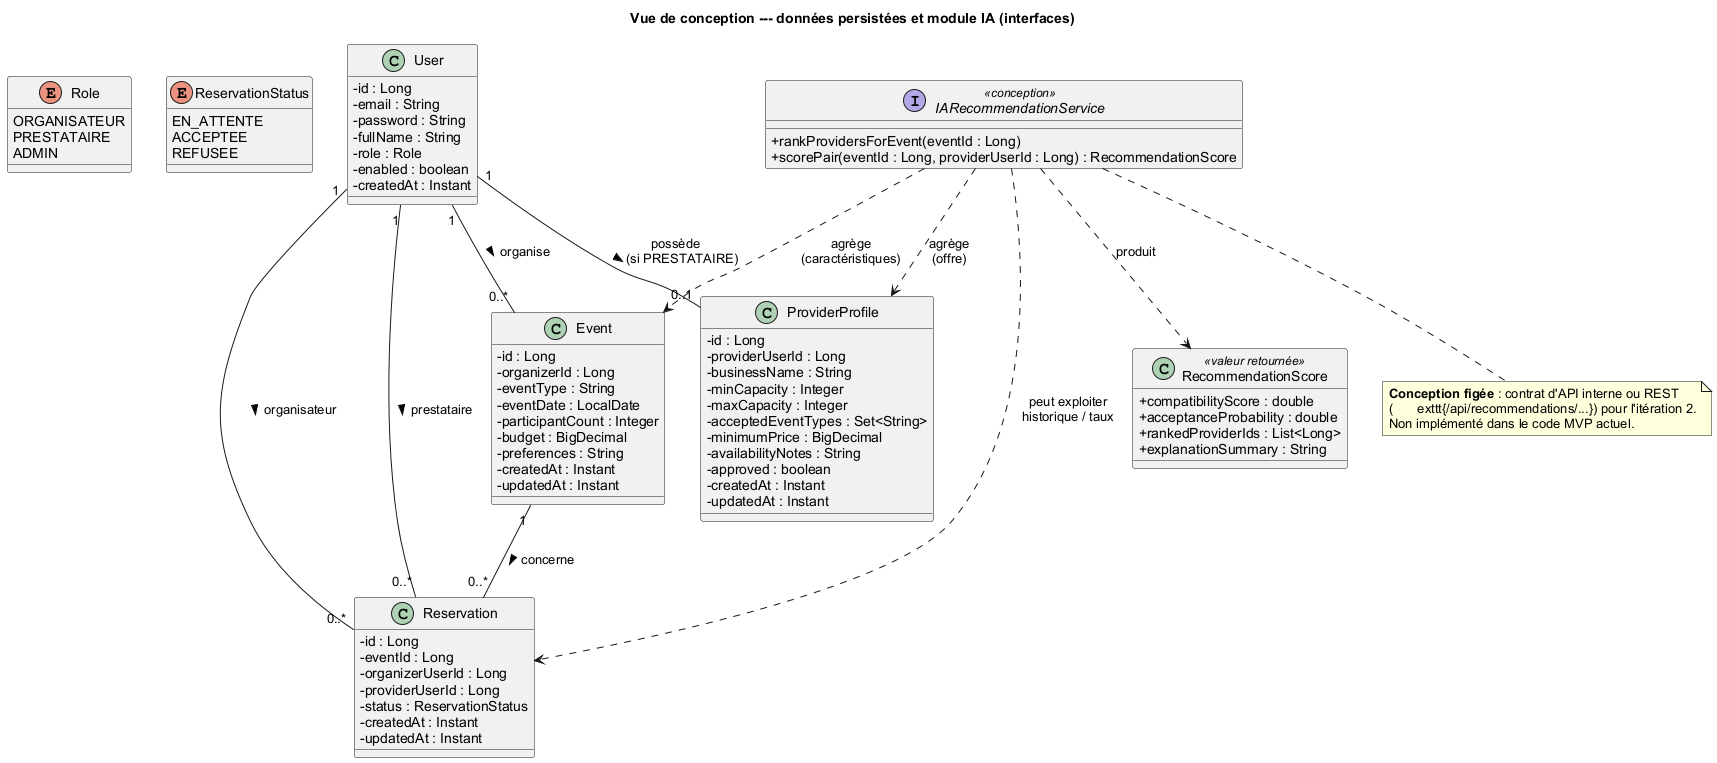
\includegraphics[width=\textwidth]{classes_metier.png}
  \caption{Classes métier persistées et service de recommandation (\texttt{RecommendationScore}, interface)}
  \label{fig:cl}
\end{figure}

\section{Diagramme de séquence --- Demande de réservation}

\begin{figure}[H]
  \centering
  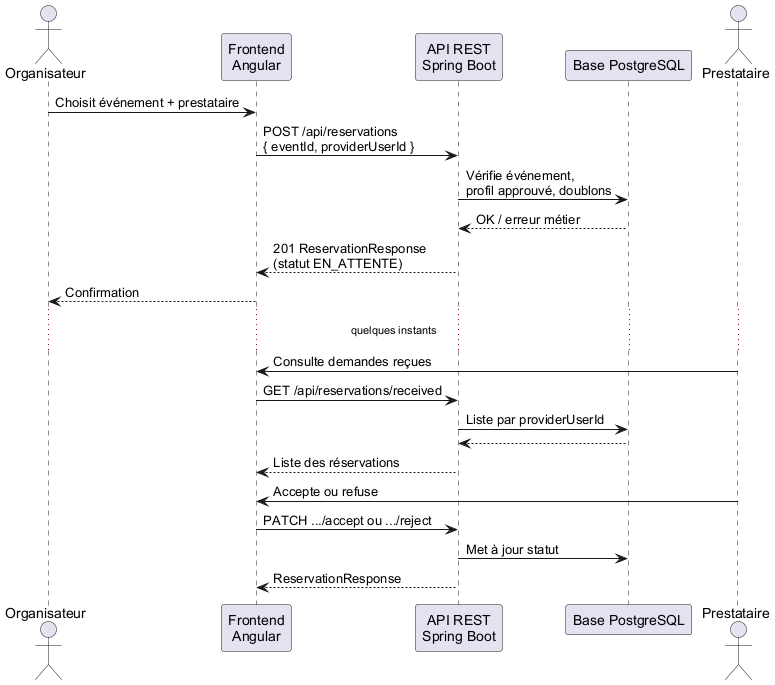
\includegraphics[width=0.95\textwidth]{sequence_demande_reservation.png}
  \caption{Séquence : création et traitement d'une réservation}
  \label{fig:seq}
\end{figure}

\section{Diagramme de séquence --- Recommandations}

\begin{figure}[H]
  \centering
  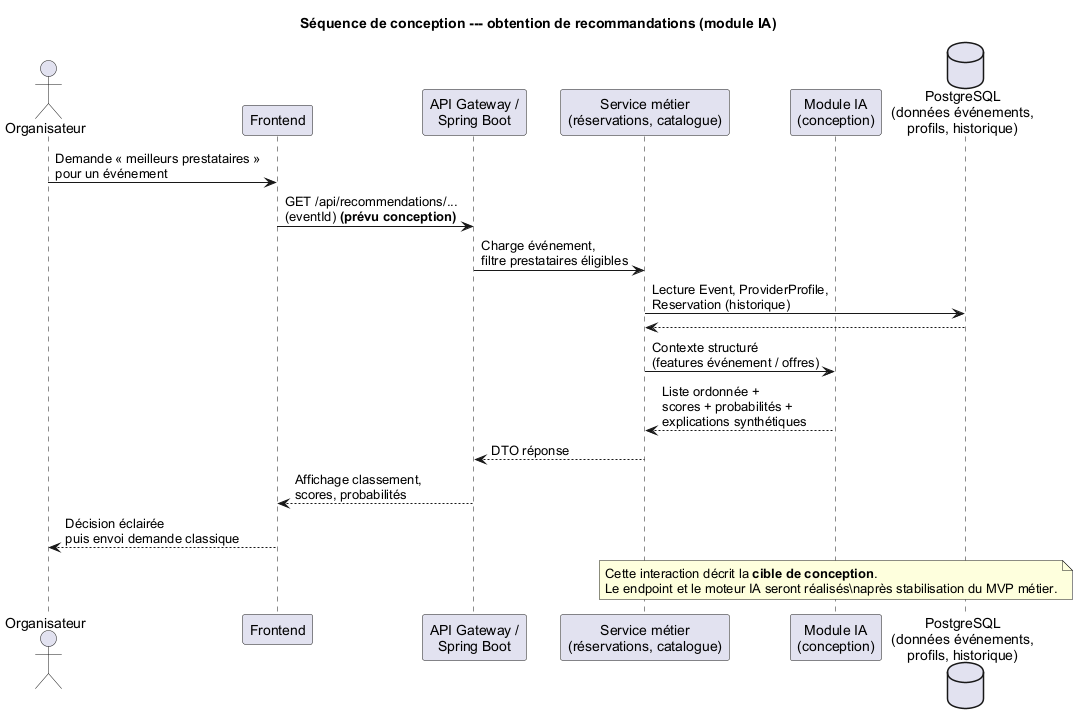
\includegraphics[width=\textwidth]{sequence_matching_ia.png}
  \caption{Séquence : consultation des recommandations et des scores (module d'intelligence artificielle)}
  \label{fig:seqia}
\end{figure}

%==================================================
\chapter{Architecture et environnement technique}
\label{chap:archi}

\section{Vue d'ensemble}

L'application adopte une architecture client-serveur : client Angular ; serveur Spring Boot exposant les ressources sous le préfixe \texttt{/api/} ; base PostgreSQL pour la persistance.

\section{Module d'intelligence artificielle dans l'architecture}

Le sous-système intelligent suit une architecture en deux temps : \textbf{Spring Boot} assure la sécurité, l'accès PostgreSQL et la constitution du paquet d'entrée (événement, profils prestataires validés, compteurs d'historique des réservations). Ce paquet est transmis par HTTP au service \textbf{FastAPI} (Python), qui calcule les scores et les textes d'explication et renvoie une liste structurée au backend. Celui-ci la relaye au client Angular via \texttt{/api/recommendations/...}. Le répertoire \texttt{ai/python-service} contient le code du microservice ; la configuration de l'URL est centralisée dans \texttt{application.yml} (\texttt{recommendation.python.base-url}).

\section{Frontend}

L'interface est organisée par rôle ; les vues organisateur intègrent l'affichage des recommandations et des scores renvoyés par les API.

%==================================================
\chapter{Réalisation et état du code}
\label{chap:real}

\section{Backend}

Le module \texttt{com.eventmanagment.backend.recommendation} regroupe \texttt{IARecommendationService}, \texttt{RecommendationServiceImpl} (orchestration), \texttt{RecommendationController}, le DTO \texttt{RecommendationScoreResponse}, le client \texttt{PythonRecommendationClient} et, pour le mode sans Python, \texttt{LocalRecommendationScorer}. Les dépôts (\texttt{EventRepository}, \texttt{ProviderProfileRepository}, \texttt{ReservationRepository}) alimentent la requête vers FastAPI. Les autres paquets couvrent les réservations, le catalogue, l'administration, l'authentification JWT et BCrypt.

\section{Frontend}

L'application Angular charge à la demande le composant \texttt{OrganizerRecommendationsComponent}, associé au service \texttt{RecommendationService} qui appelle l'API ci-dessus. Les parcours événements, catalogue, demandes, profil prestataire et administration restent structurés comme précédemment.

\section{Jeux de démonstration}

Des comptes de test sont documentés dans le projet afin de parcourir les trois rôles et les fonctionnalités intelligentes lors d'une démonstration.

%==================================================
\chapter{Interfaces et captures d'écran}
\label{chap:captures}

La figure~\ref{fig:ui_web} regroupe des extraits de l'interface web publique et d'authentification du produit.

\begin{figure}[H]
  \centering
  \begin{subfigure}[b]{0.48\textwidth}
    \centering
    
\includegraphics[width=\linewidth]{ui_accueil.jpg}
    \caption{Page d'accueil}
    \label{fig:ui_home}
  \end{subfigure}
  \hfill
  \begin{subfigure}[b]{0.48\textwidth}
    \centering
    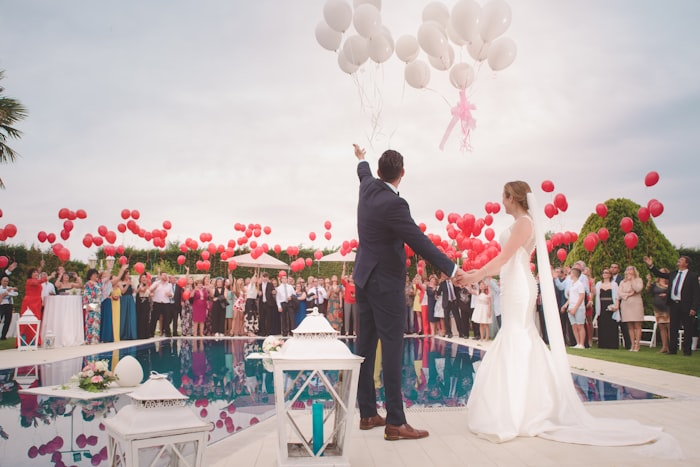
\includegraphics[width=\linewidth]{ui_types_evenements.jpg}
    \caption{Présentation des types d'événements}
    \label{fig:ui_types}
  \end{subfigure}

  \vspace{0.8em}

  \begin{subfigure}[b]{0.48\textwidth}
    \centering
    
\includegraphics[width=\linewidth]{ui_connexion.jpg}
    \caption{Formulaire de connexion}
    \label{fig:ui_auth}
  \end{subfigure}
  \caption{Extraits de l'interface utilisateur (site public et authentification)}
  \label{fig:ui_web}
\end{figure}

\noindent
L'espace organisateur inclut également l'écran \emph{Recommandations} (menu latéral), qui présente le tableau classé et les explications associées à chaque prestataire pour l'événement sélectionné. Une capture de cet écran peut être ajoutée au dossier \texttt{figures/captures/} sous le nom \texttt{ui\_recommandations.png} et insérée ici si le rapport doit illustrer explicitement ce volet.

%==================================================
\chapter{Sécurité}

L'authentification repose sur des jetons JWT ; les mots de passe sont stockés de façon hachée (BCrypt). L'autorisation est assurée par rôle ; les recommandations ne sont accessibles qu'aux comptes organisateur et pour les événements qui leur appartiennent. Des règles métier complètent ces mécanismes (par exemple limitation de certaines opérations sensibles sur les comptes administrateurs).

%==================================================
\chapter{Bilan}

\section{Conception}

La conception fonctionnelle, les modèles UML et l'architecture présentés couvrent l'ensemble du système : gestion événementielle, réservations, administration et module d'intelligence artificielle.

\section{Réalisation}

La plateforme livrée offre un ensemble cohérent sur le plan technique et fonctionnel : sécurité, parcours par rôle, services métier et intégration du volet intelligent dans la chaîne de valeur de l'organisateur.

%==================================================
\chapter*{Conclusion générale}
\addcontentsline{toc}{chapter}{Conclusion générale}

\noindent
Ce projet de fin d'études a permis de concevoir et de réaliser une plateforme événementielle couvrant la mise en relation, les réservations, l'administration et l'aide à la décision par intelligence artificielle. Les diagrammes UML et les captures d'écran illustrent la cohérence entre la modélisation, l'architecture et l'interface utilisateur.

\end{document}
